\documentclass[preview, border=20pt]{standalone}

% --- Packages ---
\usepackage[utf8]{inputenc}
\usepackage[T1]{fontenc}
\usepackage{amsmath, amssymb, amsfonts}
\usepackage{graphicx}
\usepackage{hyperref}
\usepackage{cite}
\usepackage{titlesec}
\usepackage{booktabs}
\usepackage{tikz}
\usepackage{varwidth}
\usepackage{float}
\usetikzlibrary{calc,angles,quotes}

\begin{document}

% --- Title Information ---
\title{Kinematic Modelling and MATLAB-Based Analysis of the Dobot Magician Lite Robot Arm}
\author{Ezekiel, Olomije \and Moskovitch, Yosef \and Nastase, Radu Emilian \and Oxley, John \and Raj, Shubham}
\date{}

\maketitle

\begin{abstract}
This project develops and validates a MATLAB implementation of the forward and
inverse kinematics for the Dobot Magician Lite. By simplifying the robot's
mechanical constraints into a 4-degree-of-freedom serial model, the system
provides accurate positioning, Jacobian-based singularity analysis, and robust
workspace validation.
\end{abstract}

\section{Introduction}
Robot manipulators are widely used across industrial, medical and educational
domains because of their precision, repeatability and programmability
\cite{siciliano2009}. Common applications include pick-and-place operations,
assembly lines, welding, painting, and laboratory automation. In educational
environments, robotic arms such as the Dobot Magician Lite are used for
teaching robotics concepts including kinematics, control, and programming
\cite{siciliano2009}.

The Dobot Magician Lite is a desktop serial manipulator consisting of four
revolute joints (J1--J4), forming an articulated robotic arm structure
\cite{siciliano2009}. It operates in both joint and Cartesian coordinate
systems, enabling flexible motion control and trajectory planning. The robot
supports multiple motion modes \cite{dobotManual} such as point-to-point (PTP),
linear (MOVL), and arc-based trajectories, making it suitable for both academic
and practical applications \cite{siciliano2009}.

From a classification perspective, the Dobot Magician Lite can be categorized
as a serial articulated robot arm. Compared to parallel manipulators, serial
manipulators offer a larger workspace and greater flexibility, but may suffer
from lower stiffness and accumulated positioning errors. Compared to SCARA
robots, the Dobot provides greater vertical flexibility but may have reduced
speed and precision in planar tasks.

The Dobot Magician Lite is particularly suitable for educational use because of
its low cost, ease of programming and compact desktop form \cite{dobotManual}.
However, limitations include restricted payload capacity (250 g), limited reach
(340 mm), and lower industrial-grade precision compared to high-end robotic
systems \cite{dobotManual}.

The aim of this project was to develop an analytical and MATLAB-based model of
the Dobot Magician Lite and to evaluate its forward kinematics, inverse
kinematics, Jacobian, singularities and validation behaviour.

\subsection*{List of Symbols}
\begin{itemize}
    \item $\theta_1$ -- base rotation angle
    \item $\theta_2$ -- shoulder joint angle
    \item $\theta_3$ -- elbow joint angle
    \item $\theta_4$ -- end-effector rotation angle
    \item $L_1, L_2, L_3$ -- main arm link lengths
\end{itemize}

\section{Kinematic Modelling}

\subsection{Robot configuration and assumptions}
The kinematic model therefore treats the robot as a 4R serial manipulator, with
$\theta_1$ describing base rotation, $\theta_2$ and $\theta_3$ defining planar
arm motion, and $\theta_4$ controlling tool orientation.

Although the physical robot includes a parallelogram mechanism
\cite{dobotManual} that helps maintain end-effector orientation, the kinematic
model used in this work represents that behaviour through an equivalent passive
transformation $(-\theta_3 - \theta_2)$. This passive element is not treated as
an additional actuated degree of freedom, but only as a modelling device used to
preserve the geometric constraint.

\begin{figure}[H]
    \centering
    %\includegraphics[width=0.8\textwidth]{figure1.png}
    \caption{Appearance of the Dobot Magician Lite showing the physical arrangement of the four revolute joints used in the kinematic model. Adapted from \cite{dobotManual}}
\end{figure}

\subsection{Denavit--Hartenberg parameterisation}

\begin{figure}[H]
    \centering
    %\includegraphics[width=0.8\textwidth]{figure2.png}
    \caption{Joint coordinate system of the Dobot Magician Lite showing the four revolute joints considered in the kinematic model. Adapted from \cite{dobotManual}.}
\end{figure}

\begin{figure}[H]
    \centering
    %\includegraphics[width=0.8\textwidth]{figure3.png}
    \caption{Denavit--Hartenberg frame assignment used for the kinematic modelling of the Dobot Magician Lite manipulator.}
\end{figure}

The Denavit--Hartenberg parameter table derived from the frame assignment is given below.

\begin{table}[H]
\centering
\caption{Denavit--Hartenberg parameter table derived from the frame assignment}
\begin{tabular}{lllll}
\toprule
Link & $a_i$ (mm) & $\alpha_i$ & $d_i$ (mm) & $\theta_i$ \\
\midrule
1 - Base & 0 & 90$^\circ$ & 150 & $\theta_1$ \\
2 - Rear Arm & 150 & 0 & 0 & $\theta_2$ \\
3 - Fore Arm & 150 & 0 & 0 & $\theta_3$ \\
P - uncontrollable link & 0 & 90$^\circ$ & 0 & $-\theta_3 - \theta_2$ \\
4 - End effector & 0 & 0 & 0 & $\theta_4$ \\
\bottomrule
\end{tabular}
\end{table}

The coordinate frames were assigned according to the standard
Denavit--Hartenberg convention \cite{siciliano2009}. Each $z$-axis was aligned
with the axis of rotation of the corresponding joint, while each $x$-axis was
defined along the common normal between adjacent joint axes. The physical robot
has four revolute joints; however, an additional passive transformation was
introduced only to capture the parallelogram constraint that keeps the
end-effector orientation approximately consistent. This passive term is not an
independent joint and does not increase the number of actuated degrees of
freedom \cite{craig2005}.

The Denavit--Hartenberg convention provides a systematic framework for assigning
link parameters and deriving homogeneous transformations for serial manipulators
\cite{craig2005, denavit1955}.

\subsection{Forward kinematics}
The forward kinematics of the Dobot Magician Lite were derived using the
Denavit--Hartenberg convention. A homogeneous transformation matrix was assigned
to each joint in order to describe the position and orientation of one link
frame relative to the preceding frame. The overall transformation from the base
frame to the end-effector frame was then obtained by multiplying these matrices
sequentially \cite{craig2005, denavit1955}.

For the equivalent kinematic model used in this project, the total
transformation is written as
\[ T_{04} = A_1 A_2 A_3 A_p A_4 \]
where $A_p$ denotes the passive transformation introduced to represent the
parallelogram constraint in the physical robot. This passive term is included
only to preserve the geometric behaviour of the end-effector and does not
represent an additional actuated degree of freedom.

The final homogeneous transformation matrix provides both the orientation of the
end-effector and its Cartesian position relative to the base frame. The position
terms of this transformation were later used to derive the inverse kinematics
equations and to construct the Jacobian for velocity and singularity analysis.

TODO: This is wrong as we need L1 which is non-zero

\[
T_{04} = \begin{bmatrix}
\cos(\theta_1 + \theta_4) & 0 & \sin(\theta_1 + \theta_4) & \cos(\theta_1)(L_2 \cos(\theta_2) + L_3 \cos(\theta_2 + \theta_3)) \\
\sin(\theta_1 + \theta_4) & 0 & -\cos(\theta_1 + \theta_4) & \sin(\theta_1)(L_2 \cos(\theta_2) + L_3 \cos(\theta_2 + \theta_3)) \\
0 & 1 & 0 & h + L_2 \sin(\theta_2) + L_3 \sin(\theta_2 + \theta_3) \\
0 & 0 & 0 & 1
\end{bmatrix}
\]

\subsection{Jacobian and singularity analysis}
The Jacobian matrix relates joint rates to end-effector motion. In this work,
the geometric Jacobian was used to describe the relationship between joint
velocities and the linear and angular velocity of the end-effector, while an
analytical form was considered for singularity analysis in terms of the selected
task variables \cite{siciliano2009, spong2006}. Jacobian-based analysis is
particularly useful for identifying configurations in which the manipulator
loses mobility or becomes difficult to control.

\subsubsection*{Geometric Jacobian}
The geometric Jacobian relates the joint velocities to the linear and angular
velocity of the end effector:
\[ \begin{bmatrix} v \\ \omega \end{bmatrix} = J_g(q) \dot{q} \]

The geometric Jacobian is therefore:
\[
J_g(q) = \begin{bmatrix}
-r \sin(\theta_1) & \cos(\theta_1)(-L_1 \sin(\theta_2) - L_2 \sin(\theta_2 + \theta_3)) & -L_2 \sin(\theta_2 + \theta_3) \cos(\theta_1) & 0 \\
r \cos(\theta_1) & \sin(\theta_1)(-L_1 \sin(\theta_2) - L_2 \sin(\theta_2 + \theta_3)) & -L_2 \sin(\theta_2 + \theta_3) \sin(\theta_1) & 0 \\
0 & L_1 \cos(\theta_2) + L_2 \cos(\theta_2 + \theta_3) & L_2 \cos(\theta_2 + \theta_3) & 0 \\
0 & -\sin(\theta_1) & -\sin(\theta_1) & 0 \\
0 & \cos(\theta_1) & \cos(\theta_1) & 0 \\
1 & 0 & 0 & 1
\end{bmatrix}
\]

Where: $\theta_1$ is the base rotation, $\theta_2$ is the shoulder joint angle,
$\theta_3$ is the elbow joint angle, $\theta_4$ is the tool rotation, $L_2$ is
the rear arm length, $L_3$ is the forearm length, $h$ is the base height offset.
Note that $L_1$ is not included in the Jacobian because it is a constant term
that does not affect the velocity mapping.

\subsubsection*{Analytical Jacobian}
The analytical Jacobian satisfies $\dot{x} = J_a(q) \dot{q}$ and is given by
\[
J_a(q) = \begin{bmatrix}
-r \sin(\theta_1) & \cos(\theta_1)(-L_1 \sin(\theta_2) - L_2 \sin(\theta_2 + \theta_3)) & -L_2 \sin(\theta_2 + \theta_3) \cos(\theta_1) & 0 \\
-r \cos(\theta_1) & \sin(\theta_1)(-L_1 \sin(\theta_2) - L_2 \sin(\theta_2 + \theta_3)) & -L_2 \sin(\theta_2 + \theta_3) \sin(\theta_1) & 0 \\
0 & L_1 \cos(\theta_2) + L_2 \cos(\theta_2 + \theta_3) & L_2 \cos(\theta_2 + \theta_3) & 0 \\
1 & 0 & 0 & 1
\end{bmatrix}
\]
The base offset $h$ appears in the forward kinematics of $z$, but it does not appear in the Jacobian because it is a constant term. Its derivative with respect to all joint variables is zero.

\subsubsection*{Singularities}
A singularity occurs when the determinant of the analytical Jacobian becomes zero:
\[ \det(J) = L_1 L_2 \sin(\theta_3) r = 0 \]
This expression shows that singularities occur when either $\sin(\theta_3) = 0$ or $r = 0$. The condition $\sin(\theta_3) = 0$ corresponds to the arm being fully stretched or fully folded, so that the links become collinear. The condition $r = 0$ corresponds to the wrist lying on the base axis, where the manipulator loses motion authority in certain horizontal directions. Near these configurations, the velocity mapping becomes ill-conditioned and large joint velocities may be required to generate small end-effector motions \cite{siciliano2009, spong2006}.

\subsection{Inverse kinematics}

The inverse kinematics problem was solved using a geometric approach, because it
provides closed-form solutions and is well suited to two-link planar arm
structures \cite{mathworks2023, craig2005}.

\begin{figure}[H]
    \centering
    \begin{tikzpicture}[scale=1.5, >=stealth]
        % Title
        \node[font=\bfseries, anchor=north] at (1.5, 3.5) {X-Y Plane};

        \coordinate (O) at (0,0);
        \coordinate (X) at (3,0);
        \coordinate (Y) at (0,3);
        \coordinate (J3) at (55:2.8); % Target (r, z) in projection
        
        % Axes
        \draw[->] (-0.5,0) -- (X) node[right] {$x$};
        \draw[->] (0,-0.5) -- (Y) node[above] {$y$};

        % Link projection
        \draw[thick] (O) -- (J3) node[midway, right] {$r$};
        \node[above right] at (J3) {$(x, y)$};

        % Angle q1 from y-axis to J3
        \pic [draw, "$\theta_1$", angle eccentricity=1.5, angle radius=1cm] {angle = X--O--J3};

        \fill (O) circle (1.5pt);
        \fill (J3) circle (1.5pt);
    \end{tikzpicture}
    \caption{Top-view geometry used to compute the base joint angle $\theta_1$.}
\end{figure}

The base joint angle was obtained from the top-view projection of the target
position:
\[ \theta_1 = \operatorname{atan2}(y, x) \]
The radial distance in the horizontal plane is then $r = \sqrt{x^2 + y^2}$. The
remaining problem is reduced to a planar two-link geometry in the $r$--$z$ plane
\cite{craig2005}. A geometric inverse-kinematics method was selected because it provides
closed-form solutions and is well suited to two-link planar arm structures \cite{mathworks2023,
craig2005}.

TODO: blurb as to why atan2 plus a link to the matlab docs.

\begin{figure}[H]
    \centering
    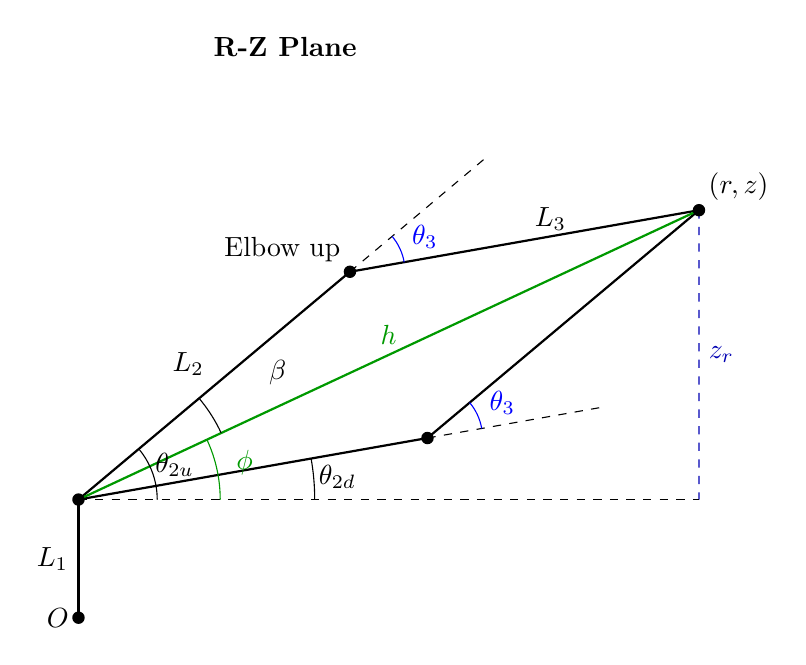
\begin{tikzpicture}[scale=1.5, >=stealth]
        % Title
        \node[font=\bfseries, anchor=north] at (1.75, 4) {R-Z Plane};
        
        % Define coordinates
        \coordinate (O) at (0,-1);
        \coordinate (J1) at (0,0);
        \coordinate (J2u) at (40:3);
        \coordinate (J2d) at (10:3);
        \coordinate (J3) at ($(J2u) + (10:3)$); % if theta2 is -30 we add that to the 40
        \coordinate (Zp) at (J3 |- J1); % Projection on horizontal

        % Draw base link
        \draw[thick] (O) -- (J1) node[midway, left] {$L_1$};
        
        % Draw links
        \draw[thick] (J1) -- (J2u) node[midway, above left] {$L_2$};
        \draw[thick] (J2u) -- (J3) node[midway, above right] {$L_3$};
        \draw[thick] (J1) -- (J2d) node[midway, above left] {};
        \draw[thick] (J2d) -- (J3) node[midway, above right] {};
        
        % Target point
        \node[above right] at (J3) {$(r, z)$};
        \node[left] at (O) {$O$};
        \node[above left] at (J2u) {Elbow up};

        
        % Distance h (hypotenuse)
        \draw[thick, green!60!black] (J1) -- (J3) node[midway, above] {$h$};
        
        % Vertical z_r
        \draw[blue!70!black, dashed] (J3) -- (Zp) node[midway, right] {$z_r$};

        % Horizontal axes
        \draw[dashed] (J1) -- (Zp);

        % Extension for theta3
        \coordinate (Ext) at ($(J1)!1.5!(J2u)$);
        \draw[dashed] (J2u) -- (Ext);
        \coordinate (Extd) at ($(J1)!1.5!(J2d)$);
        \draw[dashed] (J2d) -- (Extd);

        % Angles
        \pic [draw, "$\theta_{2u}$", angle eccentricity=1.3, angle radius=1cm] {angle = Zp--J1--J2u};
        \pic [draw, "$\theta_{2d}$", angle eccentricity=1.1, angle radius=3cm] {angle = Zp--J1--J2d};
        \pic [draw, green!60!black, "$\phi$", angle eccentricity=1.2, angle radius=1.8cm] {angle = Zp--J1--J3};
        \pic [draw, "$\beta$", angle eccentricity=1.5, angle radius=2.0cm] {angle = J3--J1--J2u};
        
        % theta3 angle from extension of L2 to L3
        \pic [draw, blue, "$\theta_3$", angle eccentricity=1.5, angle radius=0.7cm] {angle = J3--J2u--Ext};
        \pic [draw, blue, "$\theta_3$", angle eccentricity=1.5, angle radius=0.7cm] {angle = Extd--J2d--J3};
        % Joint dots
        \fill (O) circle (1.5pt);
        \fill (J1) circle (1.5pt);
        \fill (J2u) circle (1.5pt);
        \fill (J2d) circle (1.5pt);
        \fill (J3) circle (1.5pt);
    \end{tikzpicture}
    \caption{Planar geometric construction used for the inverse kinematics derivation.}
\end{figure}

Figure 5 shows the planar geometry used to derive the shoulder and elbow solutions. Two solution branches exist for reachable targets: an elbow-up configuration and an elbow-down configuration. Accordingly, the shoulder angle may be written as
\[ \theta_2 = \phi + \beta \]
for one branch and
\[ \theta_2 = \phi - \beta \]
for the other. The elbow angle $\theta_3$ is then obtained from the corresponding trigonometric relations, giving two valid inverse-kinematics solutions for the same target position.

\section{Materials and Methods}

\subsection{Kinematic Modelling Approach}
The kinematic model of the Dobot Magician Lite was developed using the Denavit--Hartenberg (DH) convention, which provides a systematic framework for describing the spatial relationship between adjacent links. Each joint was modelled as a revolute joint, and the robot was approximated as an open kinematic chain, despite the physical presence of a four-bar linkage mechanism.

A passive link was introduced in the model to maintain the constraint that the end-effector remains parallel to the ground. This simplification allows the system to be analysed using standard serial manipulator techniques while preserving key geometric behaviour.

\subsection{Inverse Kinematics Strategy}
A geometric approach was selected for solving the inverse kinematics problem. This method was chosen due to the relatively simple structure of the robot and the availability of clear geometric relationships between joint angles and end-effector position.

The inverse kinematics solution was derived by:
\begin{itemize}
    \item First solving for the base rotation using $\theta_1 = \operatorname{atan2}(y, x)$
    \item Reducing the 3D problem into a 2D planar problem in the $(r, z)$ plane
    \item Applying trigonometric relationships and cosine law to determine $\theta_2$ and $\theta_3$
    \item Considering both elbow-up and elbow-down configurations
\end{itemize}
This approach was preferred over numerical methods due to its computational efficiency, analytical clarity, and suitability for real-time applications.

\subsection{Dynamic modelling approach}
The dynamic behaviour of the manipulator was considered using the standard rigid-body robot dynamics formulation []
\[ \tau = M(q)\ddot{q} + C(q, \dot{q})\dot{q} + G(q) \]
where $\tau$ is the vector of joint torques, $M(q)$ is the inertia matrix, $C(q, \dot{q})\dot{q}$ represents Coriolis and centrifugal effects, and $G(q)$ is the gravity vector.

In the present project, the dynamic equations were incorporated at a conceptual and modelling level to extend the kinematic model developed in MATLAB. However, a complete high-fidelity dynamic implementation was limited by the lack of detailed physical parameters such as link masses, mass centres, and inertia tensors from the manufacturer documentation \cite{siciliano2009}. Therefore, the work focused on establishing the dynamic form of the equations and explaining how such terms would be integrated into the MATLAB model for future extension.

\subsection{MATLAB Implementation}
The robot model was implemented in MATLAB using a modular approach. Individual functions were created for the Denavit--Hartenberg transformations, forward kinematics evaluation, inverse kinematics solution, Jacobian computation, and workspace validation. Symbolic computation was used where appropriate to derive compact expressions for the forward kinematics and Jacobian, which were then evaluated numerically during testing \cite{corke2017}.

The implementation was designed so that a target Cartesian position could be provided as input, the corresponding joint angles could be computed through inverse kinematics, and the resulting configuration could then be verified through forward kinematics reconstruction. Additional checks were included to detect unreachable targets and singular configurations.

\subsection{Testing Framework}
A structured testing framework was used to validate the correctness of the mathematical model and its MATLAB implementation. Forward kinematics was tested by providing known joint configurations and comparing the resulting end-effector position with the expected geometric outcome. Inverse kinematics was validated by solving for joint variables from a target Cartesian position and substituting the solution back into the forward kinematics equations.

Additional tests were used to verify singularity detection and workspace rejection for unreachable targets. Together, these checks ensured internal consistency between the analytical derivations and the computational implementation.

\section{Results and Validation}
The MATLAB model was validated using forward-kinematics, inverse-kinematics and singularity test cases. Forward kinematics was checked by comparing computed end-effector positions with expected geometric outcomes, while inverse kinematics was verified by reconstructing joint configurations from target Cartesian positions. Additional tests were used to confirm singularity detection and rejection of unreachable targets.

\begin{table}[H]
\centering
\caption{Validation of forward and inverse kinematics test results table}
\begin{tabular}{llll}
\toprule
Test case & Input & Output & Remarks \\
\midrule
Forward kinematics & $q = (0.5236, 0.7854, 0, 0)$ rad & $(x, y, z) = (0.1837, 0.1061, 0.3191)$ m & Correct position \\
Inverse kinematics & Target $(0.1837, 0.1061, 0.3191)$ m & $q = (0.5236, 0.7854, 0, 0)$ rad & Successfully reconstructed \\
Singularity test & $\theta_3 = 0$ & $\det(J) = 0$ & Correctly detected \\
Unit tests & Multiple valid/invalid cases & 11/11 tests passed & Confirms consistency \\
\bottomrule
\end{tabular}
\end{table}

The validation results show good agreement between the analytical model and the MATLAB implementation. In particular, the consistency between the forward kinematics output and the inverse kinematics reconstruction confirms that the position mapping is internally correct. The singularity and unreachable-target tests further demonstrate that the implementation correctly handles important edge cases within the robot workspace.

\begin{figure}[H]
    \centering
    %\includegraphics[width=0.8\textwidth]{figure6.png}
    \caption{Successful inverse kinematics solution using the MATLAB-based UI.}
\end{figure}

\begin{figure}[H]
    \centering
    %\includegraphics[width=0.8\textwidth]{figure7.png}
    \caption{Detection of unreachable target in inverse kinematics.}
\end{figure}

The system correctly identifies when a target position lies outside the robot's reachable workspace. In this example, the computed distance $h$ exceeds the maximum reach of the robot ($L_2 + L_3 = 0.30$ m), resulting in an error message. This demonstrates that the inverse kinematics implementation includes proper workspace validation and prevents physically invalid solutions.

\section{Discussion and Conclusion}
This project developed and validated a kinematic model of the Dobot Magician Lite using the Denavit--Hartenberg formulation and implemented the main equations in MATLAB. Forward and inverse kinematics were derived analytically, the Jacobian was obtained for differential motion analysis, and singular configurations were identified from the analytical model. The resulting MATLAB implementation was able to reproduce valid end-effector positions and reject targets lying outside the reachable workspace.

One of the main technical difficulties was representing the physical parallelogram mechanism of the robot within a tractable analytical framework. This was addressed by replacing the closed-chain behaviour with an equivalent open-chain model containing a passive transformation that preserved the essential orientation constraint without introducing an additional actuated degree of freedom. A second challenge was the derivation of inverse kinematics in a form suitable for reliable computation; this was solved by reducing the problem to a planar geometric construction in the $r$--$z$ plane. A further limitation concerned dynamics, since accurate link masses, centres of mass and inertia tensors were not available in sufficient detail from the manufacturer documentation.

Despite these limitations, the final model provides a robust analytical and computational framework for studying the motion of the Dobot Magician Lite. The results demonstrate that the model is suitable for forward kinematics, inverse kinematics, singularity detection and validation testing in MATLAB. Future work could extend the model by incorporating experimentally identified dynamic parameters, actuator constraints, joint limits and closed-loop control in order to improve realism and practical applicability.

\begin{figure}[H]
    \centering
    %\includegraphics[width=0.8\textwidth]{figure8.png}
    \caption{Principal dimensions of the Dobot Magician Lite used to support the geometric assumptions of the model. Adapted from \cite{dobotManual}.}
\end{figure}

\section{References}
\bibliographystyle{plain}
\bibliography{references}

\end{document}
